\chapter{Impedance-Based BMS}

\hspace{0.5cm}
Commercial impedance meters have a wide range of capabilities, but they are rarely used as BMS. Besides size, weight, and power-consumption, they are not designed to monitor simultaneously multiple cells in a battery. Furthermore, conventional BMS that monitor impedance measure only its amplitude at a single frequency, typically at 1 kHz, and are therefore not suitable for properly characterizing a cell mismatch. The data in Figure \ref{impedence1} and Figure \ref{impedence2} demonstrate that cell impedance is indicative of calendar aging, over-discharging, and overcharging. Characterizing the impedance of a cell requires amplitude and phase measurements at multiple frequencies. Impedance based BMS is designed for such measurements. Figure \ref{BLOCK} shows such a impedance-based BMS, Battery Internal Temperature Sensor-based BMS, or BITS-BMS. It is designed to monitor each of up to 16 cells in a multi-cell battery that generates up to 80 V and 50 Ah, with no limit on the battery discharge–charge rates. This $10\ast10$ cm unit, powered by a 6 V, 0.75A dc power supply, is a standalone unit, i.e., requires no computer control to operate. It is ON when the power supply is ON, when it starts collecting data for each cell through a 16-cell multiplexer. 

\begin{figure}[H]
	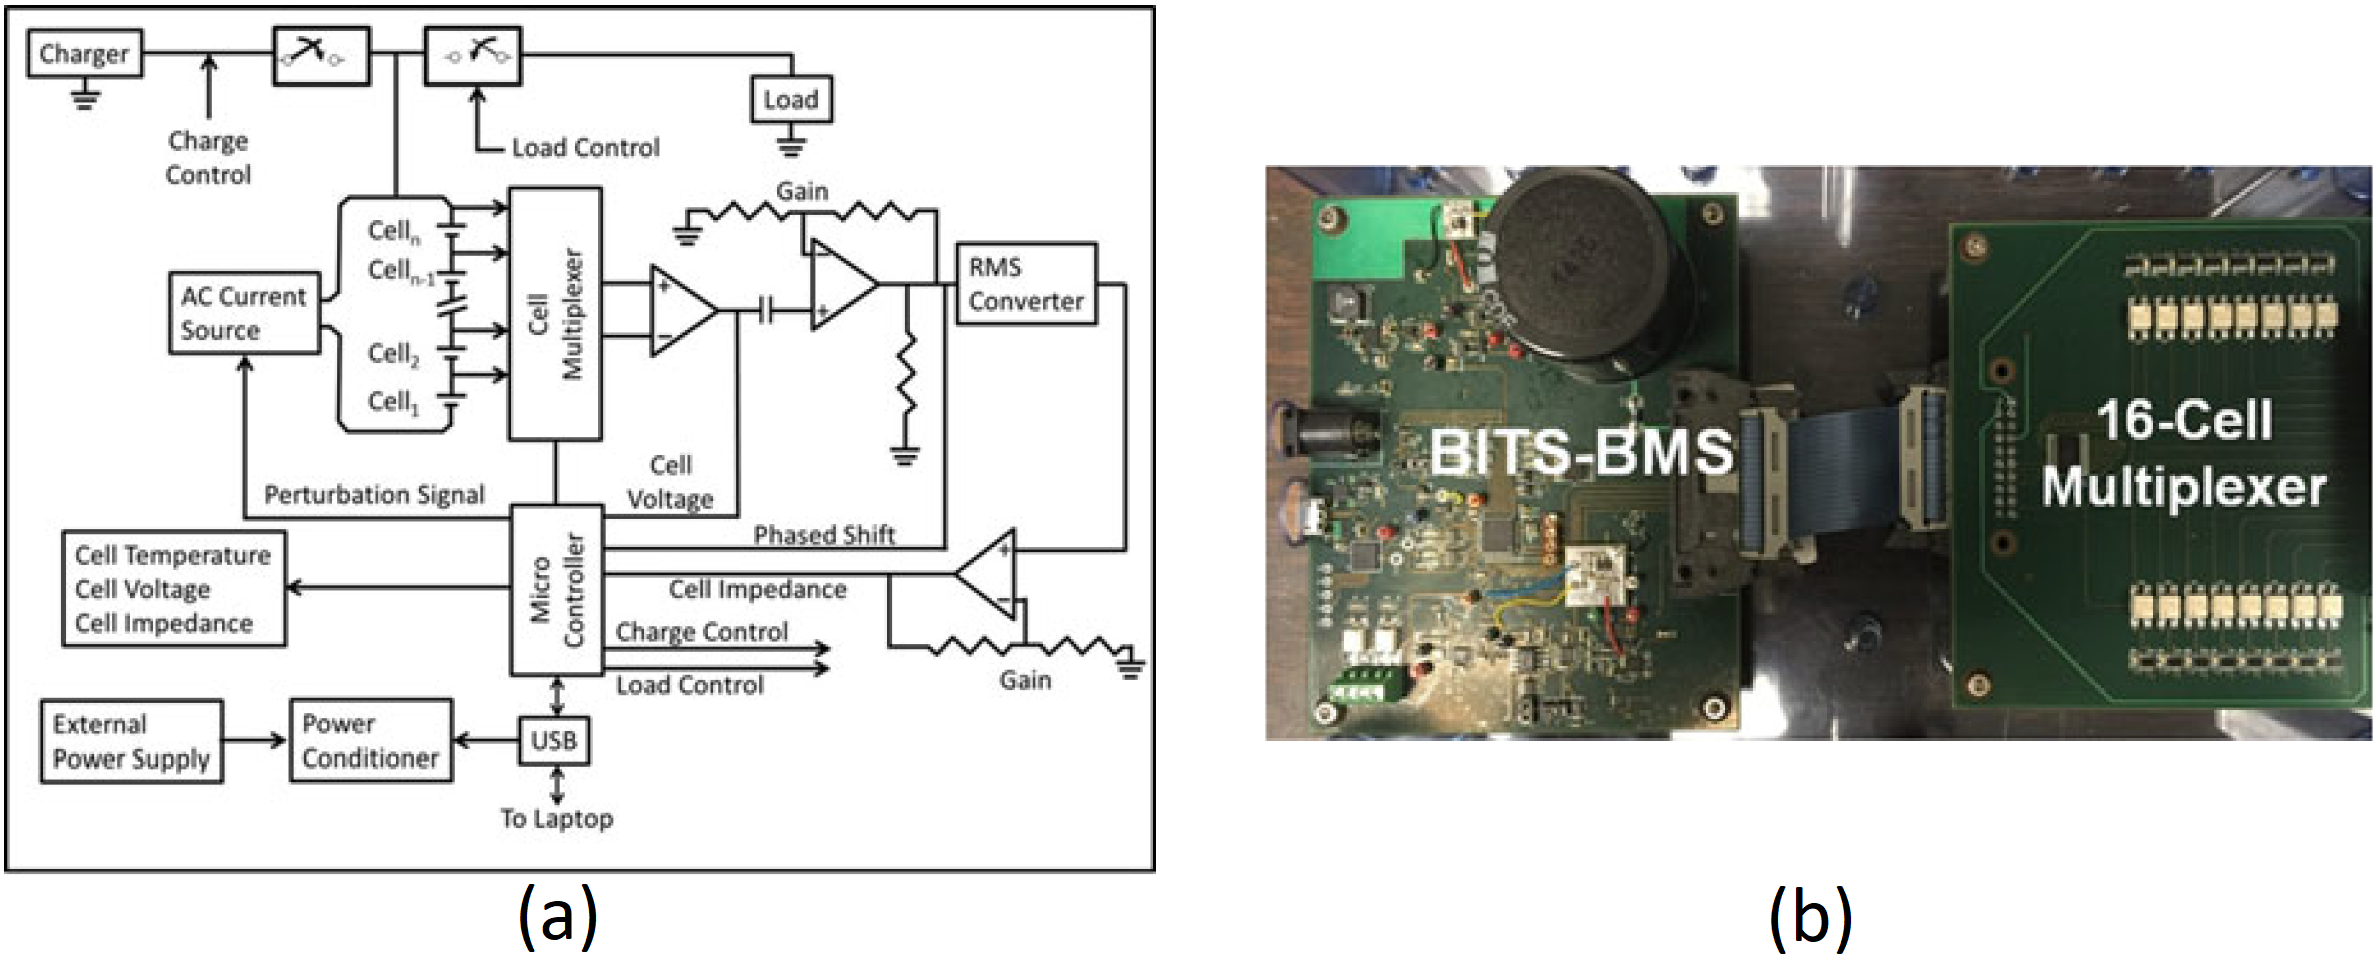
\includegraphics[width=16cm,height=6cm]{figures/BLOCK}
	\centering
	\caption{(a) Impedance-based BMS: schematic describing the main components; (b) photo of the fully operational prototype and a 16-cell multiplexer.} \label{BLOCK}
\end{figure}

\section{BITS-BMS Principle of Operation}

\hspace{0.5cm}
The BITS-BMS collects impedance data by injecting a small amplitude ac current signal of fixed amplitude (typically 100mA rms for a 50 Ah cell; or 25 mA rms for a 5 Ah cell) at multiple frequencies in the 1 Hz to 1 kHz range. This ac signal is generated via a programmable microcontroller outputting sinusoidal waveforms of fixed frequencies and fixed amplitude through a current pump. The ac current from the pump is directed toward the cells through the multiplexer, one cell at a time. The ac current perturbs the cell eliciting a voltage response. The BMS generates the perturbation signal through a constant-current source, thus ensuring identical amplitude current passes through each cell in the battery. At each frequency, the circuits following the multiplexer measure the amplitude of the resulting voltage and phase shift between the current and the voltage. The voltage amplitude is a direct measure of the cell impedance, and the phase shift is correlated to the anode temperature and cathode temperature.

\vspace{0.5cm}
The BMS has no restriction for the lower frequency cut-off. The 1 Hz to 1 kHz range adequately covers all measurements needed to manage the electrical efficiency and thermal safety in most Li-ion batteries. Each frequency or frequency range in the BMS provides specific formation: 70 Hz for the anode temperature; 10 Hz for the cathode temperature; 400-1000 Hz for electrolyte resistance and SOH; and 2 Hz for SoC. Electrolyte resistance is a ratio of cell voltage to the perturbation current, and it is measured by the BMS at a high-frequency [400 Hz in the example shown in Figure \ref{electrolyte2} (a)]. The BITS-BMS is also equipped to measure and report individual cell voltages. It rosters from one cell to the next through the multiplexer, and the measurement and reporting time per cell for all the parameters is about 22s. It has two separate features for data processing and utilization. It is programmable to send commands to control systems that regulate the current and voltages in the charging and load circuits. The user can set the desired limits on all parameters, including anode temperature, cathode temperature, cell voltage, internal resistance, SOH, and SoC of each cell. The data can also be sent from the BITS-BMS to a computer for analysis, although a computer is not required to run the BMS. The BITS-BMS will not short the wirings in the cell and the battery, and battery voltage and currents cannot influence the BMS. The upper battery voltage limit is 80 V that the BMS can handle. It can be redesigned for batteries containing more than 16 cells in series (and therefore having a higher voltage).

\section{Obtaining and Processing the Output}

\hspace{0.5cm}
BITS-BMS measures ac impedance at multiple frequencies as well as dc volts for $E_{cv}$. Between 400 Hz and 1 kHz, it measures the amplitude of the resultant ac voltage to an applied ac current, which is converted to electrolyte resistance ($R_s$ , further correlated to SOH). It also measures the impedance at a low frequency (between 1 and 2 Hz) that is correlated to SoC. The amplitude of the resultant ac voltage is measured with a 12-bit analog-to-digital converter (ADC). This binary number is sent to a processor where it is then converted into an impedance value in units of Ohms. The anode temperature and cathode temperature are measured differently from $R_s$ and SoC. Between 20 and 200 Hz, the BITS-BMS measures the phase shift that is then correlated to anode temperature. At about 10 Hz, it measures the phase shift that is then correlated to cathode temperature. 

\vspace{0.5cm}
Phase shifts (for example, at 70 and 10 Hz) are measured by comparing the zero crossing of a reference signal with the zero crossing of the return signal from the cell. The frequency of the reference signal is the same as the frequency of the perturbation current. The time interval between the zero-crossing of these two signals represents the phase difference between the perturbation signal and the resultant signal across the cell. The time interval is measured by starting and stopping a 16-bit counter which is incremented every 490nS. For 70 Hz, this yields a phase resolution of $0.0123^o$ per count. The value in the counter is read, added to an accumulator, and then reset for the next measurement. 64 readings of the counter are accumulated. Then an average is computed and the result is transmitted to an external computer (via USB), where it is displayed in units of “BITS-BMS Counts” (an arbitrary unit). Each cell model needs to be calibrated at least once against the BITS-BMS Counts (for example, at 70 and 10 Hz for measuring anode temperature and cathode temperature, respectively). During calibration, the relationship between cell temperature and the count is used to determine a fitting function that is then used to convert the counts into units of degrees Celsius. The cell voltage is also measured with the same 12-bit ADC, the resulting binary value is sent to a processor, where it is converted into units of Volts. In the context of an autonomous BITS-BMS it is not necessary to perform any conversion from the BITS-BMS internal digital values to engineering units (i.e., temperature, voltage, or ohms) but to simply use the internal digital values to make operational decisions (e.g., disconnect load, reduce or shutdown charging current).

\section{Applications of Impedance-Based BMS}

\hspace{0.5cm}
The impedance-based BITS-BMS has the ability to monitor internal temperatures (anode and cathode) in each cell, and to identify existing and emerging mismatches between cells, independent of whether the battery is at rest, being charged, or supporting a load. Such capabilities are essential to ensure safety because rising internal temperature is a precursor to thermal runaway that usually originate in a single cell (before spreading to the neighboring cell and causing conflagration). Furthermore, rising temperature in a cell skews its electrolyte resistance (high frequency), anode impedance (intermediate frequency), and/or cathode impedance (low frequency), sufficient to cause cell mismatch. 

\vspace{0.5cm}
The BITS-BMS is specifically designed to fulfill the essential safety functions, namely, monitor cell matching and SOH, and guard against excursions in $T_{int}$ and $E_{cv}$ outside pre-specified safe ranges, for every cell in a battery. In Li-ion cells, unsafe conditions such as thermal runaway are known to develop over a timescale of seconds. Therefore, the designed BITS-BMS have short reaction time. Currently, the BITS-BMS monitors safety parameters in each cell with a dwell time not exceeding 22s, monitoring only $R_s$ (at 400 Hz), anode and cathode temperatures (at 70 and 10 Hz, respectively) and $E_{cv}$. Measurements at different frequencies are sequential, monitoring only the amplitude at 400 Hz, and phase shifts at 70 and 10 Hz. Measurement of internal temperatures (anode, cathode, and electrolyte) requires calibrating the BITS-BMS output against temperature; such calibration should be performed once for each cell model. $E_{cv}$ measurements (e.g., Figure \ref{emf1}) need no calibration. The BITS-BMS outputs the data in binary format. For obtaining calibrated correlation between the binary output and internal temperatures, impedance, etc., the outputs are transferred to a computer through a USB port. For routine purposes of cell matching, controlling the charge and discharge circuits by setting upper and lower limits on the anode and cathode temperature, impedance and cell voltages, the binary outputs of the BITS-BMS are used.The BITS-BMS outputs during (dis)charge of the battery with five aged cells and one over-discharged cell are shown in Figure \ref{result}. For the five cells, the rates of change of the BMS output were nearly identical. Only the over discharged cell showed a clear and significant departure in the rate of change of the BMS output, indicative of the cell being bad.

\begin{figure}
	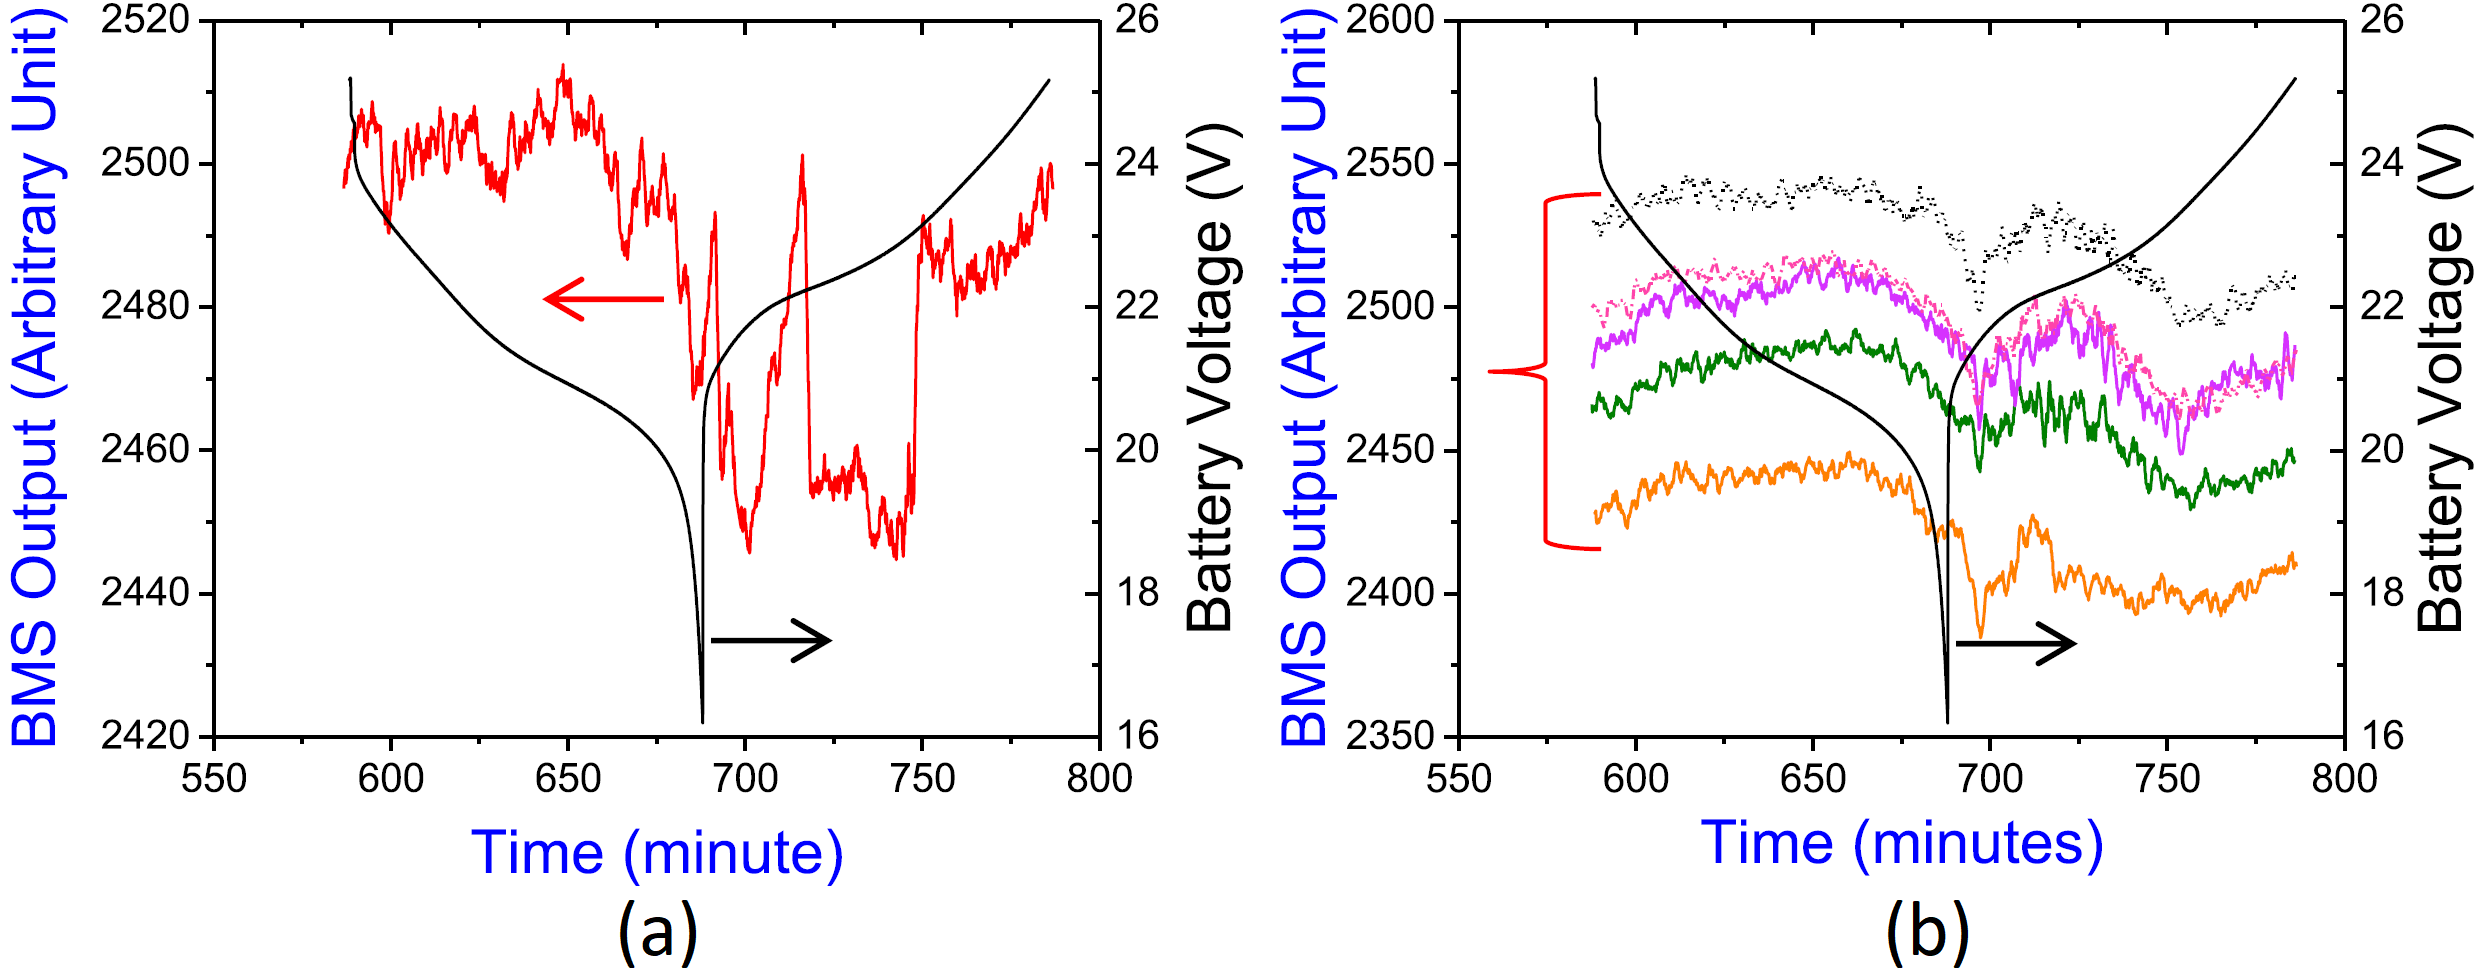
\includegraphics[width=16cm,height=6cm]{figures/result}
	\centering
	\caption{Outputs of impedance-based BITS-BMS for a six-cell battery containing five calendar-aged cells and one over-discharged cell, during a discharge–charge cycle: (a) Overdischarged cell only; (b) five calendar-aged, otherwise normal cells.} \label{result}
\end{figure}

